\section{Methodology}\label{sec:method}

We scale Xmodel-2 to 1.3\,B parameters while retaining its deployment-friendly, deep-and-thin decoder-only skeleton.
The section below details three design pillars:
(i) architecture-level $\mu$P compatibility (\S\ref{sec:arch}),
(ii) a three-phase Warmup--Stable--Decay (WSD) curriculum (\S\ref{sec:wsd}), and
(iii) FP8 mixed-precision acceleration (\S\ref{sec:fp8-detail}).

\subsection{Model Architecture}\label{sec:arch}
Xmodel-2.5 keeps the deep-and-thin decoder-only design of Xmodel-2, with the configuration in Table~\ref{tab:config}.
To preserve maximal-update dynamics across widths we apply the $\mu$P attention-logits scaling $1/d_{\text{head}}$; all other components (Pre-RMSNorm, SwiGLU) are inherited without modification.
While Xmodel-2 was trained with Flash-Attention v2, Xmodel-2.5 uses the CuDNN backend provided by Megatron-LM (no \texttt{--use-flash-attn} specified).

\begin{table}[htbp]
\centering
\small
\begin{tabular}{lc}
\toprule
\textbf{Hyper-parameter} & \textbf{Value} \\
\midrule
Hidden size & 1536 \\
Intermediate size & 3840 \\
Num of transformer layers & 48 \\
Attention heads (Q) & 24 \\
KV heads (GQA) & 8 \\
Sequence length & 3712 \\
Max position embeddings & 131072 \\
RoPE base & 500000 \\
\bottomrule
\end{tabular}
\caption{Model configuration. {\footnotesize Long-context support via 131\,K position embeddings and RoPE base 500\,K.}}
\label{tab:config}
\end{table}

\subsection{Three-Phase WSD Pre-Training}\label{sec:wsd}

The 560\,k-step Warmup--Stable--Decay (WSD) schedule consumes 1.4\,T tokens:
\begin{enumerate}
  \item \textbf{Warmup (W)}: 2\,k steps, LR linearly rises to $1.67\!\times\!10^{-3}$ (hidden) and $0.01$ (embeddings).
  \item \textbf{Stable (S1)}: 270\,k steps, batch size 3\,712$\times$480$\approx$1.78\,M tokens.
  \item \textbf{Stable (S2)}: 260\,k steps, batch size 3\,712$\times$960$\approx$3.56\,M tokens.
  \item \textbf{Decay (D)}: 20\,k steps (exponential decay), batch size $\approx$3.56\,M tokens, 66.9\,\% high-quality SFT data blended.
  \item \textbf{Long-Context Reasoning (LCR)}: 10\,k additional steps, \emph{same} 66.9\,\% SFT ratio, batch size 16\,384$\times$240$\approx$3.93\,M tokens, context length 16\,k.
\end{enumerate}

\paragraph{Optimizer ablation: AdamW $\rightarrow$ Muon.}
During the final 20\,k decay steps we perform a controlled optimizer switch: AdamW is replaced by Muon~\citep{jordan2024muon} while \emph{all other hyper-parameters remain frozen}, including the learning-rate schedule, batch size, gradient-clip, weight-decay, and the 66.9\,\% SFT data blend.
Under this single-variable change, the 13-task reasoning average rises by 4.58\,pp \emph{absolute} over an AdamW-only baseline, confirming that the gain is attributable to Muon and not to confounding factors such as data re-weighting or schedule re-tuning.
This result supports the view that early-phase stability (AdamW) can be complementarily combined with late-phase sharpness (Muon) to improve downstream performance without extra data or re-training.

\begin{figure*}[htbp]
    \centering
    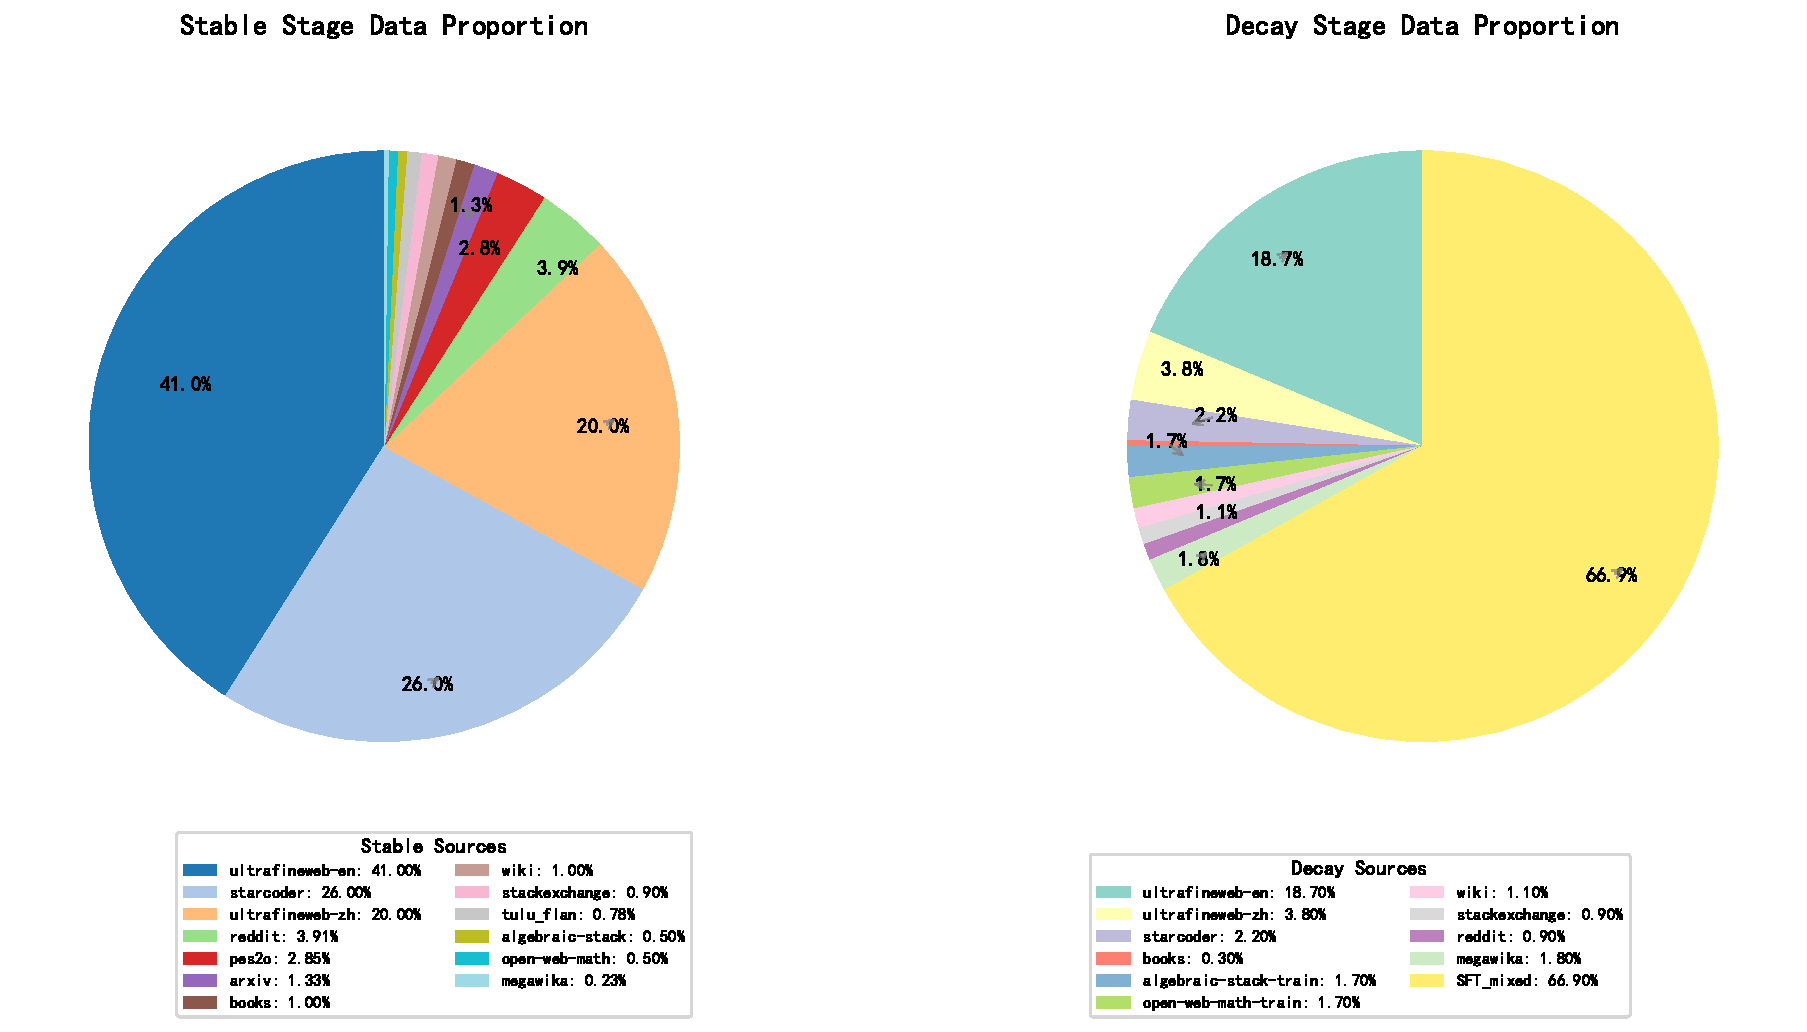
\includegraphics[width=0.95\textwidth]{figures/stable_vs_decay_enhanced.pdf}
    \caption{Data composition in the (a) Stable and (b) Decay phases of WSD LR scheduling. The Stable phase emphasizes broad pre-training data diversity, while the Decay phase focuses on high-quality instructional and SFT data to refine model capabilities.}
    \label{fig:data_composition}
\end{figure*}

\subsection{FP8 Hybrid Format \& Kernel Implementation}
\label{sec:fp8-detail}

We adopt the FP8 hybrid format implemented in NVIDIA Transformer Engine~(TE)~\cite{nvidia-transformer-engine}:
\begin{itemize}[leftmargin=*,nosep]
  \item \textbf{Forward}: E4M3 (1-4-3 exponent-mantissa) for activations;
  \item \textbf{Backward}: E5M2 (1-5-2) for gradients;
  \item \textbf{Master-weights}: kept in \texttt{bfloat16} to avoid under-flow.
\end{itemize}
TE delayed-scaling hyper-parameters: \texttt{amax-history-len}=128, \texttt{amax-compute-algo}=\texttt{max}.  
All FP8 kernels are invoked through Megatron-LM's \texttt{--transformer-impl transformer\_engine} flag;  
the corresponding GEMM, Layer-Norm and GeLU CUDA kernels are automatically selected without source-code modification. 